\subsection{Parameter Initialisation}\label{sec:parinital}
In \autoref{sec:multilayer}, the output of a neural network was calculated, however observe that the parameters $\theta = \{\text{weights, biases}\}$ were not explicitly stated, as ideal values for these variables are currently unknown. Training the neural network is used to determine the parameters; such objective can be achieved by minimising the error, which leads to \autoref{subsec:train}. 
However, these parameters should be initialised in advance of those procedures. 
Initialisation may have a major effect on the convergence of deep neural networks training, to be discussed in \autoref{sec:gradientdescent}, a feat critical to the success of the network.
Simple schemes have been identified to speed up learning, but care is needed to prevent common pitfalls. Here, a fairly basic method of initialisation is introduced. 
Firstly, the weights are assigned values randomly; this can be generated using the normal distribution with mean $0$ and variance $\nicefrac{1}{n}$ for some $n\in\mathbb{N}_1$ denoting the number of datasets. The advantages of this generation leads to a lack of symmetry for each perceptron in \autoref{fig:multi}, that is, perceptrons are discouraged in learning identically. Lastly, it is common to initialise all biases to zero as the weights defined above already provide asymmetry. 

Indeed the randomness of $\theta$ may yield a random set of meaningless outputs. However, after initialisation, the parameters can now be numerically analysed, in order to observe the error they yield. 

\subsection{Error Cost Function}\label{subsec:train}
For this article, the neural network is limited to supervised learning, that is, the desired output is already known. In particular, there exists a training dataset.

\begin{defn}
A training dataset $\mathcal{T}$ consists of input-output pairs $(X,Y)$, where $X$ is input matrix and $Y$ is the desired (target) output matrix of the network on input $X$. Then a training dataset of size $T$ is denoted $\mathcal{T}:=\set{(X_i,Y_i):1\leq i \leq T}$.
\end{defn}

As shown above, the ANN has a mapping $F:X\rightarrow \overline{Y}$ defined $F(\theta;X)=\overline{Y}$, where $F$ is the implemented transformations in forward propagation. Consider a single arbitrary element $(X,Y)\in\mathcal{T}$, then the error between the predicted output $\overline{Y}$ and the desired output $Y$ is given by the squared loss function\footnote{The square loss function is used here in preparation for the squared error cost function, however one may use the absolute loss for the absolute error cost function. } for $y\in Y$ and $\overline{y} \in\overline{Y}$,
\begin{align*}
    \mathcal{L}(Y,\overline{Y})=\sum_{i=1}^{n^{(L)}} (\overline{y}_{i}-y_i)^2,
\end{align*}
where $n^{(L)}$ is the dimensionality of the target set (ipso facto, the size of the predicted output set). However, the loss function only considers the errors produced by a single element from the dataset, hence the error cost function $\mathcal{J}$ is used to  calculate a single-valued total error by computing over the entire training data set. Similar to the activation function, there are many different functions that may be used including: Mean Squared Error (MSE) and Root Mean Square (RMS). For its simplicity and popularity, the Squared Error (SE) will be used  \parencite[]{taylorbook},
\begin{align}
    \mathcal{J}_{SE}(\theta;\mathcal{T})
    &=\frac{1}{2}\sum_{i=1}^{T} \mathcal{L}^{(i)} 
    \label{eq:squareerror},
\end{align}
where $\mathcal{L}^{(i)}$ is the loss function for the $i$-th training element of $\mathcal{T}$.

For the sake of simplicity, the size of the training dataset, $T$, will be $1$. Therefore, along with the fact that $n^{(L)}=n^{(2)}=1$ (see \autoref{fig:multi}) and $\overline{y}\in \overline{Y}=F(\theta;X)$, 
our cost function can be denoted,
\begin{align}
    \mathcal{J}:=\mathcal{J}_{SE}=\frac{1}{2}\mathcal{L}(y,\overline{y})=\frac{1}{2}(\overline{y}-y)^2 \label{eq:reducedsquareerror}.
\end{align}

Take note that the set of parameters $\theta$ in \autoref{fig:multi} is equivalent to the set $\{W^{(1)},W^{(2)}\}$, where the biases have been integrated into the weight matrices accordingly. As shown in \autoref{fig:multi}, the elements of $W^{(2)}$ have a direct implication towards the output layer. While the elements in $W^{(1)}$ have an indirect implication towards the output layer, since such elements are separated by the hidden layer. However, since both weight matrices have impacts, they both must be considered when minimising the squared error cost function. Hence, the objective function of neural network training can be represented as,
\begin{align*}
    \min_{w\in\theta} \mathcal{J}(\theta;\mathcal{T}).
\end{align*}
Now we investigate a method for minimising this objective function. 

\subsection{Gradient Descent}\label{sec:gradientdescent}
The gradient descent method, first proposed by French mathematician Augustin-Louis Cauchy in 1847, is the most widely used supervised optimisation algorithm to train neural networks. This first-order iterative algorithm calculates the local minimum of a differentiable function, whence minimising the function. Gradient descent is useful for complicated models that neural networks aim to tackle due to the ability to process multi-variable functions. Some of the types of gradient descent include: batch gradient descent, all of the training examples are processed for each iteration of gradient descent; stochastic gradient descent, a single training example is processed for each iteration. 

\begin{defn} The gradient matrix of a differentiable function $f:\mathbb{R}^{m\times n}\rightarrow \mathbb{R}$ at a point $W\in\mathbb{R}^{m\times n}$ for some $m,n\in\mathbb{N}_1$, denoted $\nabla f$, is defined
\begin{equation}
    \nabla f(W)=
    \arraycolsep=1pt\def\arraystretch{1.5}
    \begin{bmatrix}
            \frac{\partial f}{\partial w_{1,1}} &  \frac{\partial f}{\partial w_{1,2}} & \dots & \frac{\partial f}{\partial w_{1,n}} \\
            \frac{\partial f}{\partial w_{2,1}} &  \frac{\partial f}{\partial w_{2,2}} & \dots & \frac{\partial f}{\partial w_{2,n}} \\
            \vdots & \vdots & \ddots & \vdots \\
            \frac{\partial f}{\partial w_{m,1}} &  \frac{\partial f}{\partial w_{m,2}} & \dots & \frac{\partial f}{\partial w_{m,n}}
        \end{bmatrix},
\end{equation}
    that is, the partial derivative of $f(W)$ with respect to $w_{i,j}$ is the $(i,j)$-th element in $\nabla f(W)$. Moreover, for $w\in W$ the notation is,
\begin{align*}
    \nabla_w f=\frac{\partial f}{\partial w}.
\end{align*}
\end{defn}
Consider the initial point of parameters $\theta^{[0]}$ that was initialised in \autoref{sec:parinital},  where the bracketed-superscript denotes the iteration. Then given a training set $\mathcal{T}$, the update policy for the parameters in gradient descent is as follows \parencite{Zhanggradient},
\begin{align}
    \theta^{[t+1]}=\theta^{[t]}-\eta \nabla_\theta \mathcal{J}(\theta^{[t]};\mathcal{T}), \label{eq:iteration}
\end{align}
 for every iteration $t\in\mathbb{N}_0$, where $\eta$ is the learning rate. The role and significance of the learning rate is discussed below in \autoref{sec:learningrate}. Note  $-\eta \nabla \mathcal{J}_\theta( \theta^{[t]};\mathcal{T}) = \Delta \theta^{[t]}$, that is, the direction the parameters are updated is by an $\eta$-scaled negative gradient matrix. 

Now consider the optimal set of parameters, $\Hat{\theta}$, given by
\begin{align*}
    \Hat{\theta} =\arg\min_{\theta\in\mathbb{R}^d} \mathcal{J}(\theta;\mathcal{T}),
\end{align*}
for some dimension $d$. Assume an appropriate $\eta$ is chosen. Then gradient descent algorithm converges and terminates for some iteration $t^*\in \mathbb{N}_0$ such that 
\begin{align*}
    || \mathcal{J}(\theta^{[t^*]};\mathcal{T}) - \mathcal{J}(\Hat{\theta};\mathcal{T}) || < \epsilon
\end{align*}
for all $\epsilon>0$, that is, 
$
    \lim_{t \rightarrow t^*} \theta^{[t]} \approx \hat{\theta}
$ \parencite{sum8789696}.
While the proof of convergence of the gradient descent is beyond the scopes of this article, \textcite{converge} provides evidence of this assertion. It is only required to know that the derivative of cost function with respect to the parameters does indeed converge, and converges when $t\rightarrow t^*$.  Such $t^*$ does not necessarily need be known, as the following algorithm \parencite[8]{Zhanggradient} will terminate appropriately. 
\begin{algorithm}[H]
    \caption{Batch Gradient Descent}
    \begin{algorithmic}[1]
        \Require{$\mathcal{T}, \eta$}
        \Ensure{ $\theta^{[t^*]}$ }
        \State $t\leftarrow 0$
        \State Initialise parameters
        \State Fix $\epsilon > 0$
        \While {$|| \mathcal{J}(\theta^{[t]};\mathcal{T}) - \mathcal{J}(\Hat{\theta};\mathcal{T}) || > \epsilon$}
            \ForAll {$(X,Y)\in\mathcal{T}$}
                \ForAll {$w \in \theta$}
                    \State $w\leftarrow w-\eta \nabla_w \mathcal{J}(\theta^{[t]};X,Y)$
                   
                \EndFor
            \EndFor
            \State $t\leftarrow t+1$
        \EndWhile 
    \end{algorithmic}
    \label{alg:grad}
\end{algorithm}
Therefore, it remains to calculate $\nabla_w \mathcal{J}$ for  \cref{alg:grad}. 
\subsubsection{Computing gradient with respect to \texorpdfstring{$W^{(2)}$}{W⁽²⁾}}
In preparation of computing the gradients, the following theorem is required.
\begin{thm}[Chain Rule for Composite Functions]
Suppose that $y=f(x)$ and $x=g(t)$ are differentiable functions of $t$. Then $y=f\circ g (t)$ is a differentiable function of $t$ and
\begin{align*}
    \frac{\partial y}{\partial t} = 
    \frac{\partial y}{\partial x}
    \frac{\partial x}{\partial t}.
\end{align*}
\end{thm}
\begin{proof}
Proven in \textcite{Herman2021Chain}.
\end{proof}
Consider an arbitrary element $w^{(2)}_{q} \in W^{(2)}$ for any $0\leq q\leq n^{(1)}$. Then using gradient descent, parameter $w^{(2)}_{q}$ can be optimized, that is, calculating the minima of the SE function with respect to $w^{(2)}_{q}$,
\begin{align*}
    \frac{\partial \mathcal{J}_{SE}}{\partial w^{(2)}_{q}} 
    &= \frac{\partial}{\partial w^{(2)}_{q}} \sbr[4]{\frac{1}{2}\sum_{r=1}^{n^{(2)}} {(a^{(2)}_r-y_r)^2}}\\
     &=\sum_{r=1}^{n^{(2)}}  \left[{(a^{(2)}_r-y_r)} \frac{\partial}{\partial w^{(2)}_{q}} \sbr[3]{a_r^{(2)}-y_r}\right].
\end{align*}
Using the argument for \autoref{eq:reducedsquareerror},
\begin{align}
    \frac{\partial \mathcal{J}}{\partial w^{(2)}_{q}} 
    &=(a^{(2)}-y) \frac{\partial}{\partial w^{(2)}_{q}} \sbr[3]{a^{(2)}-y}.
    \label{eq:costdiff}
\end{align}
Observe the role of the constant `$\nicefrac{1}{2} $' in $\mathcal{J}$ is for convenience, to enable a simpler differentiation, but the sum of squared errors does not necessarily need such coefficient in order to compute the error\footnote{In \autoref{eq:squareerror}, one would need to linearly scale accordingly to find the error without the constant coefficient.}. Additionally, observe that $a^{(2)}$ is the only variable of $w^{(2)}_{q}$; oppose to the fact $\nicefrac{\partial y}{\partial w^{(2)}_{q}} = 0$. The results are simplified with the use of the chain rule,
\begin{align}
    \frac{\partial \mathcal{J}}{\partial w^{(2)}_q} 
    &=(a^{(2)}-y) \frac{\partial a^{(2)}}{\partial w^{(2)}_{q}} \nonumber \\
    &= (a^{(2)}-y) \sigma'(z^{(2)}) \frac{\partial z^{(2)}}{\partial w^{(2)}_q} .\label{eq:costdiff2}
\end{align}
Recall \autoref{eq:zee}, and investigating the partial derivative required,
\begin{align*}
\frac{\partial z^{(2)}}{\partial w^{(2)}_q} &= \frac{\partial}{\partial w^{(2)}_q} \sbr[3]{(W^{(2)})^\top A^{(1)}} \\
&=\frac{\partial}{\partial w^{(2)}_q} \sbr[3]{w^{(2)}_q a^{(1)}_q}\\
&= a^{(1)}_q.
\end{align*}
Thus \autoref{eq:costdiff2} becomes,
\begin{align}
    \frac{\partial \mathcal{J}}{\partial w^{(2)}_q} 
    &= (a^{(2)}-y) \sigma'(z^{(2)}) a^{(1)}_q. \label{eq:eleven}
\end{align}
This indeed is the desired derivative, however notation found in literature for this equation is commonly simplified to the `delta form'. The purpose will become more apparent when calculating the gradient of $\mathcal{J}$ with respect to $W^{(1)}$.
\begin{defn}
Consider an $L$-layer neural network and let $0\leq i \leq n^{(\ell)}$ denote $i$-th neuron at the $\ell$-th layer. Similarly, let $0\leq j \leq n^{(\ell-1)}$ denote $j$-th neuron at the $(\ell-1)$-th layer. Then,
\begin{align*}
   \delta^{(\ell)}_i \equiv \frac{\partial \mathcal{J}}{\partial z^{(\ell)}_i},
\end{align*}
where $\delta$ is representing the error at each neuron $i$ in layer $\ell$ for $1\leq \ell \leq L$.
Then, for the output layer ($\ell=L$),
\begin{align*}
    \delta^{(L)}_i = (a^{(L)}_i-y_i)\sigma'(z^{(L)}_i),
\end{align*}
where $\delta$ is representing the error in the $i$-th output \parencite{PIETILA2012987}.
\label{defn:deltaform}
Hence, the \textit{delta form} of derivative the cost error with respect to the weights of the output layer is given by
\begin{equation}
    \frac{\partial \mathcal{J}}{\partial w^{(L)}_{i,j}} = \delta^{(L)}_i a^{(L-1)}_{j}. \label{eq:DELTAFORM}
\end{equation}
\end{defn}
In a nutshell, \autoref{eq:DELTAFORM} calculates the contribution of each $w^{(L)}_{p,q}$ adds to the error signal by weighting the error by the magnitude of the previous layer's output activation. 

Hence, in Step 5 for \cref{alg:grad} (gradient descent algorithm),
\begin{align*}
    w^{(2)}_{q} & \leftarrow  w^{(2)}_q - \eta \nabla_{w^{(2)}_q} \mathcal{J} \\
    &\leftarrow  w^{(2)}_q - \eta \frac{\partial \mathcal{J}}{\partial w^{(2)}_q} \\
    &\leftarrow  w^{(2)}_{q} - \eta \delta^{(2)} a^{(1)}_q.
\end{align*}
\begin{rem}
Recall that, $a^{(1)}_j=1$ for the bias $w^{(2)}_j$, for $j=0$. Thus \autoref{eq:eleven} gives, 
$$ \frac{\partial \mathcal{J}}{\partial w^{(2)}_0} = \delta^{(2)}. $$
Therefore, the bias is only updated by the information on or after its respective layer. 
\end{rem}


\subsubsection{Computing gradient with respect to \texorpdfstring{$W^{(1)}$}{W⁽¹⁾}}
Now the issue arises on how the partial derivatives of different layers than the output layer can be calculated. 
Notice that computing gradient with respect to $W^{(2)}$ for back-propagation only goes back upto the hidden layer in \autoref{fig:multi}. Consequently, the indirect weights remain unchanged, however the error back-propagation can be extended all the way back to the input layer by repeating the process successively. Then, similar to above,
\begin{align}
    \frac{\partial \mathcal{J}}{\partial w^{(1)}_{p,q}} 
    %&= \frac{\partial}{\partial w^{(1)}_{i,j}} \sbr[3]{\frac{1}{2}\sum_{k=1}^K {(a^{(2)}_k-t_k)^2}}\\
    %&=\sum_{k=1}^K {(a^{(2)}_k-t_k)} \frac{\partial}{\partial w^{(1)}_{i,j}} \sbr[3]{a_k^{(2)}-t_k} \\
    &={(a^{(2)}-{y})} \sigma'(z^{(2)}) \frac{\partial z^{(2)}}{\partial w^{(1)}_{p,q}}. \label{eq:fairytail}
\end{align}
Using the chain rule to compute,
\begin{align}
    \frac{\partial z^{(2)}}{\partial w^{(1)}_{p,q}} 
    &= \frac{\partial z^{(2)}}{\partial a^{(1)}_{q}} \frac{\partial a^{(1)}_{q}}{\partial w^{(1)}_{p,q}} \nonumber\\
    &=w_{q}^{(1)}\sigma'(z^{(1)}_q) \frac{\partial z_q^{(1)}}{\partial w^{(1)}_{p,q}} \nonumber \\
    &=w_{q}^{(1)}\sigma'(z^{(1)}_q) a^{(0)}_p \nonumber \\
    &=w_{q}^{(1)}\sigma'(z^{(1)}_q) x_p \label{eq:hello}.
\end{align}
Hence, combining \autoref{eq:hello} and \autoref{eq:fairytail},
\begin{align}
    \frac{\partial \mathcal{J}}{\partial w^{(1)}_{p,q}} &= {(a^{(2)}-{y})} \sigma'(z^{(2)})w_{q}^{(1)}\sigma'(z^{(1)}_q) x_p. \nonumber
\end{align}
Again, the equation will be simplified to the delta form.
Consider the following error term equation by \cref{defn:deltaform} and the chain rule \parencite{artifical},
\begin{align*}
    \delta^{(\ell)}_i \equiv  \frac{\partial \mathcal{J}}{\partial z^{(\ell)}_{i}} 
    = \sum_{j=1}^{n^{(\ell+1)}} 
    \frac{\partial \mathcal{J}}{\partial z^{(\ell+1)}_{j}} 
    \frac{\partial z^{(\ell+1)}_{j}}{\partial z^{(\ell)}_{i}},
\end{align*}
for $1\leq \ell\leq L-1$ and $1\leq i \leq n^{(\ell)}$. Then, investigating the partial derivatives individually,
\begin{align*}
     \frac{\partial z^{(\ell+1)}_{j}}{\partial z^{(\ell)}_{i}} 
     &= \frac{\partial}{\partial z^{(\ell)}_{i}} \left[ \sum_{i=1}^{n^{(\ell)}} w_{i,j}^{(\ell)}a^{(\ell)}_i \right] \\
     &= \frac{\partial}{\partial z^{(\ell)}_{i}} \left[ w_{i,j}^{(\ell)}a^{(\ell)}_i \right] \\
     &= w_{i,j}^{(\ell)} \sigma'(z^{(\ell)}_{i}).
\end{align*}
And by \cref{defn:deltaform}, 
\begin{align*}
     \frac{\partial \mathcal{J}}{\partial z^{(\ell+1)}_{j}} &\equiv \delta_j^{(\ell+1)}.
\end{align*}
Therefore, the error $\delta$ is determined as follows for any layer before the output layer,
\begin{align*}
    \delta^{(\ell)}_i &= \sigma'(z_i^{(\ell)}) \sum_{j = 1}^{n^{(\ell+1)}} \delta_j^{(\ell+1)}w_{i,j}^{(\ell+1)},
\end{align*}
for $1\leq \ell \leq L-1$. This is known as the back-propagation formula. Hence the delta form for the partial derivative is,
\begin{align}
    \frac{\partial \mathcal{J}}{\partial w^{(1)}_{p,q}} 
    &=\left(\delta^{(2)} w^{(2)}_{q} \sigma'(z^{(1)}_q)\right) x_p 
    =\delta^{(1)}_q x_p. \label{eq:hellokitty}
\end{align}
Thus, the parameters in the hidden layer are updated as follows, 
\begin{align*}
    w^{(1)}_{p,q}
    &\leftarrow  w^{(1)}_{p,q} - \eta \delta^{(1)}_q x_p.
\end{align*}

\subsection{Learning Rate}\label{sec:learningrate}
We have discussed the importance of parameters such as weights and biases, known as machine-learnable parameters. However, the learning rate $\eta$ is a configurable hyper-parameter\footnote{Hyper-parameter is a parameter used to control the learning process. } used in the training of neural networks. Unlike machine-learnable parameters, which are derived from the learning process, the learning rate must be predefined to tweak the model's output as well as to monitor how the algorithms learn.
%Evidently by Fig. \ref{fig:multilearn}, the learning rate is significant. 

\begin{figh}
        \begin{subfigure}[h]{0.48\linewidth}
    \centering
    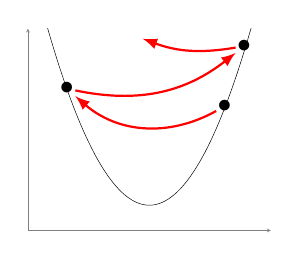
\begin{tikzpicture}[scale=.45]
        \begin{axis}[   
            grid=minor,  
            ticks=none,
            xmin=0,
            xmax=4,
            axis x line=middle,
            ymax=.8,
            ymin=0,
            axis y line=left,
            no markers,
            axis line style=gray,
            xlabel style=gray,
            ylabel style=gray,
        ]
            \addplot[black,mark=none,samples=200,domain=0:10,] (x,{(x/2-1)^2+.1});
            %\addplot[dashed,black,mark=none,samples=200,domain=0:10,] (x,{.7*x-1.8});
        \end{axis}
        
        \node[inner sep=1mm] (A) at (5.55,3.5){};
        \node[inner sep=1mm] (B) at (1.1,4){};
        \node[inner sep=1mm] (C) at (6.1,5.2){};
        \node[inner sep=1mm] (D) at (3,5.5){};
        
        \draw[-latex,red, thick] (A) edge[bend left=35] (B);
        \draw[-latex,red, thick] (B) edge[bend right=25] (C);
        \draw[-latex,red, thick] (C) edge[bend left=15] (D);
        
        \node[inner sep=-.2mm] at (A){$\bullet$};
        \node[inner sep=-.2mm] at (B){$\bullet$};
        \node[inner sep=-.2mm] at (C){$\bullet$};
\end{tikzpicture}
    \caption{}
    \label{fig:learnveryhigh}
\end{subfigure}
\hfill
\begin{subfigure}[h]{0.48\linewidth}
    \centering
    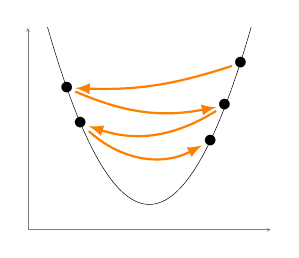
\begin{tikzpicture}[scale=.45]
        \begin{axis}[   
            grid=minor,  
            ticks=none,
            xmin=0,
            xmax=4,
            axis x line=middle,
            ymax=.8,
            ymin=0,
            axis y line=left,
            no markers,
            axis line style=gray,
            xlabel style=gray,
            ylabel style=gray
        ]
            \addplot[black,mark=none,samples=200,domain=0:10,] (x,{(x/2-1)^2+.1});
            %\addplot[dashed,black,mark=none,samples=200,domain=0:10,] (x,{.7*x-1.8});
        \end{axis}
        
        \node[inner sep=1mm] (A) at (6,4.7){};
        \node[inner sep=1mm] (B) at (1.1,4){};
        \node[inner sep=1mm] (C) at (5.55,3.5){};
        \node[inner sep=1mm] (D) at (1.48,3){};
        \node[inner sep=1mm] (E) at (5.15,2.5){};
        
        \draw[-latex,orange, thick] (A) edge[bend left=10] (B);
        \draw[-latex,orange, thick] (B) edge[bend right=17] (C);
        \draw[-latex,orange, thick] (C) edge[bend left=25] (D);
        \draw[-latex,orange, thick] (D) edge[bend right=35] (E);
        
        \node[inner sep=-.2mm] at (A){$\bullet$};
        \node[inner sep=-.2mm] at (B){$\bullet$};
        \node[inner sep=-.2mm] at (C){$\bullet$};
        \node[inner sep=-.2mm] at (D){$\bullet$};
        \node[inner sep=-.2mm] at (E){$\bullet$};
\end{tikzpicture}
    \caption{}
    \label{fig:learnhigh}
\end{subfigure}
\vspace{2mm}
\begin{subfigure}[h]{0.48\linewidth}
    \centering
    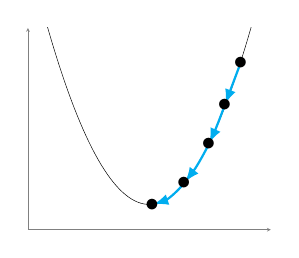
\begin{tikzpicture}[scale=.45]
        \begin{axis}[   
            grid=minor,  
            ticks=none,
            xmin=0,
            xmax=4,
            axis x line=bottom,
            ymax=.8,
            ymin=0,
            axis y line=left,
            no markers,
            axis line style=gray,
            xlabel style=gray,
            ylabel style=gray
        ]
            \addplot[black,mark=none,samples=200,domain=0:10,] (x,{(x/2-1)^2+.1});
            %\addplot[dashed,black,mark=none,samples=200,domain=0:10,] (x,{.7*x-1.8});
        \end{axis}
        
        \node[inner sep=-.2mm] (A) at (6,4.7){};
        \node[inner sep=-.2mm] (B) at (5.55,3.5){};
        \node[inner sep=-.2mm] (C) at (5.1,2.4){};
        \node[inner sep=-.2mm] (D) at (4.4,1.3){};
        \node[inner sep=-.2mm] (E) at (3.5,.7){};
        
        \draw[-latex,cyan, thick] (A) -- (B);
        \draw[-latex,cyan, thick] (B) edge[bend left=2] (C);
        \draw[-latex,cyan, thick] (C) edge[bend left=5] (D);
        \draw[-latex,cyan, thick] (D) edge[bend left=15] (E);
        
        \node[inner sep=-.2mm] at (A){$\bullet$};
        \node[inner sep=-.2mm] at (B){$\bullet$};
        \node[inner sep=-.2mm] at (C){$\bullet$};
        \node[inner sep=-.2mm] at (D){$\bullet$};
        \node[inner sep=-.2mm] at (E){$\bullet$};
        
	\end{tikzpicture}
    \caption{}
    \label{fig:learnopt}
\end{subfigure}
\hfill
\begin{subfigure}[h]{0.48\linewidth}
    \centering
    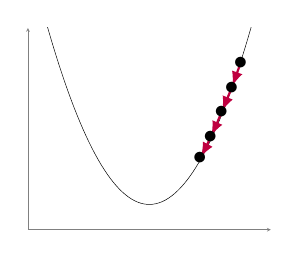
\begin{tikzpicture}[scale=.45]
        \begin{axis}[   
            grid=minor,  
            ticks=none,
            xmin=0,
            xmax=4,
            axis x line=bottom,
            ymax=.8,
            ymin=0,
            axis y line=left,
            no markers,
            axis line style=gray,
            xlabel style=gray,
            ylabel style=gray
        ]
            \addplot[black,mark=none,samples=200,domain=0:10,] (x,{(x/2-1)^2+.1});
            %\addplot[dashed,black,mark=none,samples=200,domain=0:10,] (x,{.7*x-1.8});
        \end{axis}
        
        \node[inner sep=-.2mm] (A) at (6,4.7){};
        \node[inner sep=-.2mm] (B) at (5.75,4){};
        \node[inner sep=-.2mm] (C) at (5.46,3.3){};
        \node[inner sep=-.2mm] (D) at (5.15,2.6){};
        \node[inner sep=-.2mm] (E) at (4.85,2){};
        
        \draw[-latex,purple, thick] (A) -- (B);
        \draw[-latex,purple, thick] (B) -- (C);
        \draw[-latex,purple, thick] (C) edge[bend left=1] (D);
        \draw[-latex,purple, thick] (D) edge[bend left=2] (E);
        
        \node[inner sep=-.2mm] at (A){$\bullet$};
        \node[inner sep=-.2mm] at (B){$\bullet$};
        \node[inner sep=-.2mm] at (C){$\bullet$};
        \node[inner sep=-.2mm] at (D){$\bullet$};
        \node[inner sep=-.2mm] at (E){$\bullet$};
        
	\end{tikzpicture}
    \caption{}
    \label{fig:learnlow}
\end{subfigure}
        \caption{(a) Very high $\eta$ causes divergences (b) High $\eta$ causes overshooting (c) Optimal $\eta$ converges to minima (d)  Low $\eta$ converges slowly towards minima.}
        \label{fig:multilearn}
\end{figh}
    
As like the activation and cost functions, the learning rate is given by a function of preference.  \textcite{wu2019demystifying} states choosing an appropriate learning rate can be difficult, as depicted in \autoref{fig:multilearn}.
As if $\eta$ is small, then due to the minor changes made to the weights of each update the rate of convergence will be slow, whence require more training epochs (one cycle through the full training dataset). In contrast, if $\eta$ is large, then due to rapid changes, the risk of overshooting arises but require fewer training epochs. In some cases this may lead to the variables diverging from the optimal and in others result in sub-optimality. Hence any desirable learning rate must have such trade offs.
    
The constant learning rate is a baseline default function for neural network frameworks (e.g.  Caffe)\footnote{Caffe is an open source deep learning framework originally developed at University of California, Berkeley.}. An optimum constant learning rate for a model cannot be calculated with analysis methods on a given dataset, however, a good sufficient learning rate can be achieved by trial and error \parencite{wu2019demystifying}.  In general, a popular and naive starting point is taking a relatively very small constant learning rate, for instance $\eta := 1\mathrm{e}{-1} = 0.1$. Then, decrement the exponential per simulation of the neural network until a suitable learning rate is produced, e.g. $1\mathrm{e}{-2}= 0.01$, $1\mathrm{e}{-3}= 0.001$, etc. 
%But of course alternative functions can be used instead of the default, for example, the fixed step size (decaying) learning rate. 

\subsection{Limitations of Gradient Descent}
While gradient descent has been shown to be very useful for achieving the objective function, there are indeed limitations:

\begin{itemize}[leftmargin=*]
    \item As previously stated, a suitable learning rate must be chosen to ensure the success of a parameter update policy. 
    \item If the error cost function has a large number of local minima, there is no guarantee that the process will find the global minimum \parencite{298667}.
    The gradient descent algorithm, in particular, does not distinguish between local and global minima, because once a process reaches a minima, it is unable to escape (given that the learning rate is not sufficiently large enough to exceed the size of the ditch). 
    \item The optimal parameters the process yields is dependable on the initialisation of the parameters, that is, let $\Bar{\theta}$ and $\Tilde{\theta}$ be distinct parameter initialisations, then $\Bar{\theta}^{[t^*]}$ and $\Tilde{\theta}^{[t^*]}$ may or may not be identical. This difference between the two optimal parameters the process yields can be as small as the $\epsilon$ in \cref{alg:grad} or can be a consequence of the limitation above, the parameters have converged into different minima.
\end{itemize}
